\documentclass{standalone}
\usepackage{tikz}
\begin{document}
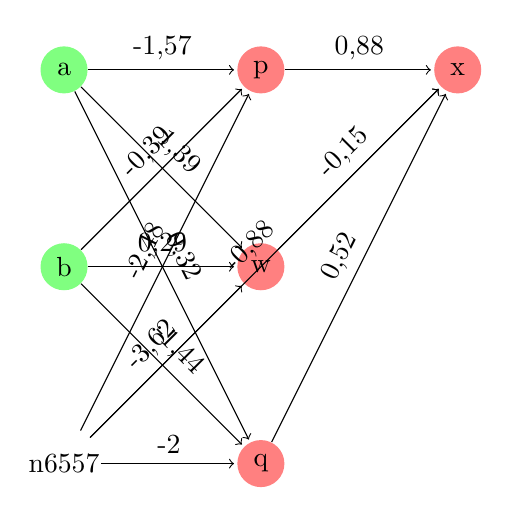
\begin{tikzpicture}[shorten >=1pt,->,draw=black!,node distance=2.5cm]
\tikzstyle{neuron}=[circle,fill=black!25,minimum size=17pt,inner sep=0pt]
\tikzstyle{constant}=[neuron, fill=white!50];
\tikzstyle{sigmoid}=[neuron, fill=red!50];
\tikzstyle{identity}=[neuron, fill=green!50];
\node [identity] (a) {a};
\node [identity,below of=a] (b) {b};
\node [constant,below of=b] (n6557) {n6557};
\node [sigmoid,right of=a] (p) {p};
\node [sigmoid,below of=p] (w) {w};
\node [sigmoid,below of=w] (q) {q};
\node [sigmoid,right of=p] (x) {x};
\path[every node/.style={sloped,anchor=south,auto=false}]
(n6557) edge node {-2} (q)
(n6557) edge node {-3,62} (w)
(n6557) edge node {-2,48} (p)
(n6557) edge node {-0,88} (x)
(p) edge node {0,88} (x)
(w) edge node {-0,15} (x)
(q) edge node {0,52} (x)
(b) edge node {0,29} (w)
(b) edge node {-0,39} (p)
(b) edge node {-1,44} (q)
(a) edge node {-1,57} (p)
(a) edge node {0,32} (q)
(a) edge node {1,39} (w)
;\end{tikzpicture}
\end{document}